\begin{subfigure}[t]{0.9\textwidth}
        \centering
        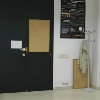
\includegraphics[scale=0.7]{figures/lasiesta/frame0}
        \hfill
        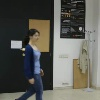
\includegraphics[scale=0.7]{figures/lasiesta/frame100}
        \hfill
        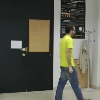
\includegraphics[scale=0.7]{figures/lasiesta/frame190}
        \hfill
        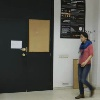
\includegraphics[scale=0.7]{figures/lasiesta/frame250}
        \hfill
        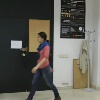
\includegraphics[scale=0.7]{figures/lasiesta/frame270}
        \caption{Original LASIESTA frames.}
    \end{subfigure}
    \\ \bigskip
    \begin{subfigure}[t]{0.9\textwidth}
        \centering
        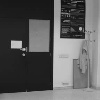
\includegraphics[scale=0.7]{figures/LASIESTA-PLAIN-DIFFERENCING/frame0}
        \hfill
        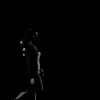
\includegraphics[scale=0.7]{figures/LASIESTA-PLAIN-DIFFERENCING/frame100}
        \hfill
        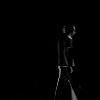
\includegraphics[scale=0.7]{figures/LASIESTA-PLAIN-DIFFERENCING/frame190}
        \hfill
        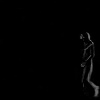
\includegraphics[scale=0.7]{figures/LASIESTA-PLAIN-DIFFERENCING/frame250}
        \hfill
        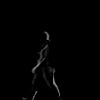
\includegraphics[scale=0.7]{figures/LASIESTA-PLAIN-DIFFERENCING/frame270}
        \caption{Frame Differencing with no HE.}
    \end{subfigure}
    \\ \bigskip
    \begin{subfigure}[t]{0.9\textwidth}
        \centering
        \includegraphics[scale=0.7]{figures/LASIESTA-PLAIN-MEAN/frame0}
        \hfill
        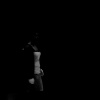
\includegraphics[scale=0.7]{figures/LASIESTA-PLAIN-MEAN/frame100}
        \hfill
        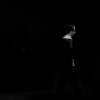
\includegraphics[scale=0.7]{figures/LASIESTA-PLAIN-MEAN/frame190}
        \hfill
        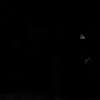
\includegraphics[scale=0.7]{figures/LASIESTA-PLAIN-MEAN/frame250}
        \hfill
        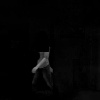
\includegraphics[scale=0.7]{figures/LASIESTA-PLAIN-MEAN/frame270}
        \caption{Mean Filter with no HE.}
    \end{subfigure}
    \\ \bigskip
    \begin{subfigure}[t]{0.9\textwidth}
        \centering
        \includegraphics[scale=0.7]{figures/LASIESTA-PLAIN-GAUSSIAN/frame0}
        \hfill
        \includegraphics[scale=0.7]{figures/LASIESTA-PLAIN-GAUSSIAN/frame100}
        \hfill
        \includegraphics[scale=0.7]{figures/LASIESTA-PLAIN-GAUSSIAN/frame190}
        \hfill
        \includegraphics[scale=0.7]{figures/LASIESTA-PLAIN-GAUSSIAN/frame250}
        \hfill
        \includegraphics[scale=0.7]{figures/LASIESTA-PLAIN-GAUSSIAN/frame270}
        \caption{Gaussian Average with no HE.}
    \end{subfigure}
    \\ \bigskip
    \begin{subfigure}[t]{0.9\textwidth}
        \centering
        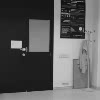
\includegraphics[scale=0.7]{figures/LASIESTA-CKKS-DIFFERENCING/frame0}
        \hfill
        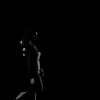
\includegraphics[scale=0.7]{figures/LASIESTA-CKKS-DIFFERENCING/frame100}
        \hfill
        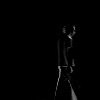
\includegraphics[scale=0.7]{figures/LASIESTA-CKKS-DIFFERENCING/frame190}
        \hfill
        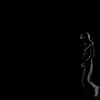
\includegraphics[scale=0.7]{figures/LASIESTA-CKKS-DIFFERENCING/frame250}
        \hfill
        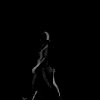
\includegraphics[scale=0.7]{figures/LASIESTA-CKKS-DIFFERENCING/frame270}
        \caption{Frame Differencing with CKKS.}
    \end{subfigure}
    \\ \bigskip
    \begin{subfigure}[t]{0.9\textwidth}
        \centering
        \includegraphics[scale=0.7]{figures/LASIESTA-CKKS-MEAN/frame0}
        \hfill
        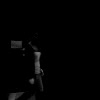
\includegraphics[scale=0.7]{figures/LASIESTA-CKKS-MEAN/frame100}
        \hfill
        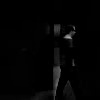
\includegraphics[scale=0.7]{figures/LASIESTA-CKKS-MEAN/frame190}
        \hfill
        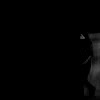
\includegraphics[scale=0.7]{figures/LASIESTA-CKKS-MEAN/frame250}
        \hfill
        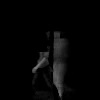
\includegraphics[scale=0.7]{figures/LASIESTA-CKKS-MEAN/frame270}
        \caption{Mean Filter with CKKS.}
    \end{subfigure}
    \\ \bigskip
    \begin{subfigure}[t]{0.9\textwidth}
        \centering
        \includegraphics[scale=0.7]{figures/LASIESTA-CKKS-GAUSSIAN/frame0}
        \hfill
        \includegraphics[scale=0.7]{figures/LASIESTA-CKKS-GAUSSIAN/frame100}
        \hfill
        \includegraphics[scale=0.7]{figures/LASIESTA-CKKS-GAUSSIAN/frame190}
        \hfill
        \includegraphics[scale=0.7]{figures/LASIESTA-CKKS-GAUSSIAN/frame250}
        \hfill
        \includegraphics[scale=0.7]{figures/LASIESTA-CKKS-GAUSSIAN/frame270}
        \caption{Gaussian Average with CKKS.}
    \end{subfigure}
